% iaus2esa.tex -- sample pages for Proceedings IAU Symposium document class
% (based on v1.0 cca2esam.tex)
% v1.04 released 17 May 2004 by TechBooks
%% small changes and additions made by KAvdH/IAU 4 June 2004
% Copyright (2004) International Astronomical Union

\NeedsTeXFormat{LaTeX2e}

\documentclass{iau_FM}
\usepackage{graphicx}
\usepackage{natbib}

\title[Gaussian processes for stellar rotation]
{Stellar rotation period inference with Gaussian processes}

\author[Ruth Angus, Suzanne Aigrain \& Daniel Foreman-Mackey]
{Ruth Angus$^1$,
Susanne Aigrain$^1$
\and Daniel Foreman-Mackey$^2$}

\affiliation{$^1$Subdepartment of Astrophysics, University of Oxford, Oxford,
	UK \\
email: {\tt ruth.angus@astro.ox.ac.uk}, {\tt suzanne.aigrain@astro.ox.ac.uk} \\[\affilskip]
$^2$Sagan Fellow, Department of Astronomy, University of Washington, Seattle
\\ email: {\tt danfm@uw.edu}}

\pubyear{2015}
\setcounter{page}{1}
\jname{Astronomy in Focus, Volume 1}
\editors{Piero Benvenuti, ed.}
\begin{document}

\maketitle

% \begin{abstract}
The light curves of spotted, rotating stars are often non-sinusoidal and
Quasi-Periodic (QP) and a strictly periodic sinusoid is therefore not
a representative generative model.
Ideally, a physical model of the stellar surface would be conditioned on the
data, however the parameters of such models can be highly degenerate.
Instead, we use an appropriate {\it effective} model: a Gaussian Process (GP)
with a QP covariance kernel function.
% \begin{equation}
% 	k_{i, j} = A \exp \left[ - \frac{\sin^2(\pi(x_i-x_j)/P)} \
% 	{2g^2}-\frac{(x_i-x_j)^2}{2l^2}\right],
% \end{equation}
% with
By modelling the covariance matrix of the light curve with a QP GP, we remain
agnostic about model choice, whilst sampling directly from the posterior
probability distribution function of the periodic parameter and marginalising
over the other kernel hyperparameters.
We simulated 300 light curves with a range of rotation periods and spot
lifetimes and attempted to recover the rotation periods using three methods:
our GP method, a sine-fitting periodogram method and an AutoCorrelation
Function (ACF) method.
% Function (ACF) method \citep{amy}.
The posterior probability distribution of the rotation period parameter was
sampled using the affine invariant ensemble MCMC sampler, {\tt emcee}
% \footnote{
% Foreman-Mackey {\it et al.}, 2013, PASP, 125, 306}
and the
GP operations were performed using the {\tt george} python package
% \footnote{https://github.com/dfm/george}.
This method produces rotation periods that are more precise than the
periodogram and both more accurate and precise than the ACF method.
Furthermore, the improvement is expected to be even more dramatic when applied
to real, noisy {\it Kepler} light curves, since the GP method is well suited to
modelling rotation signals and correlated noise simultaneously.

\keywords{Stars: rotation, Methods: data analysis, Methods: statistical,
techniques:photometric}
% \end{abstract}

% \firstsection % if your document starts with a section,
%               % remove some space above using this command.
% \section{Introduction}

\begin{figure}[b]
% \vspace*{-2.0 cm}
\begin{center}
	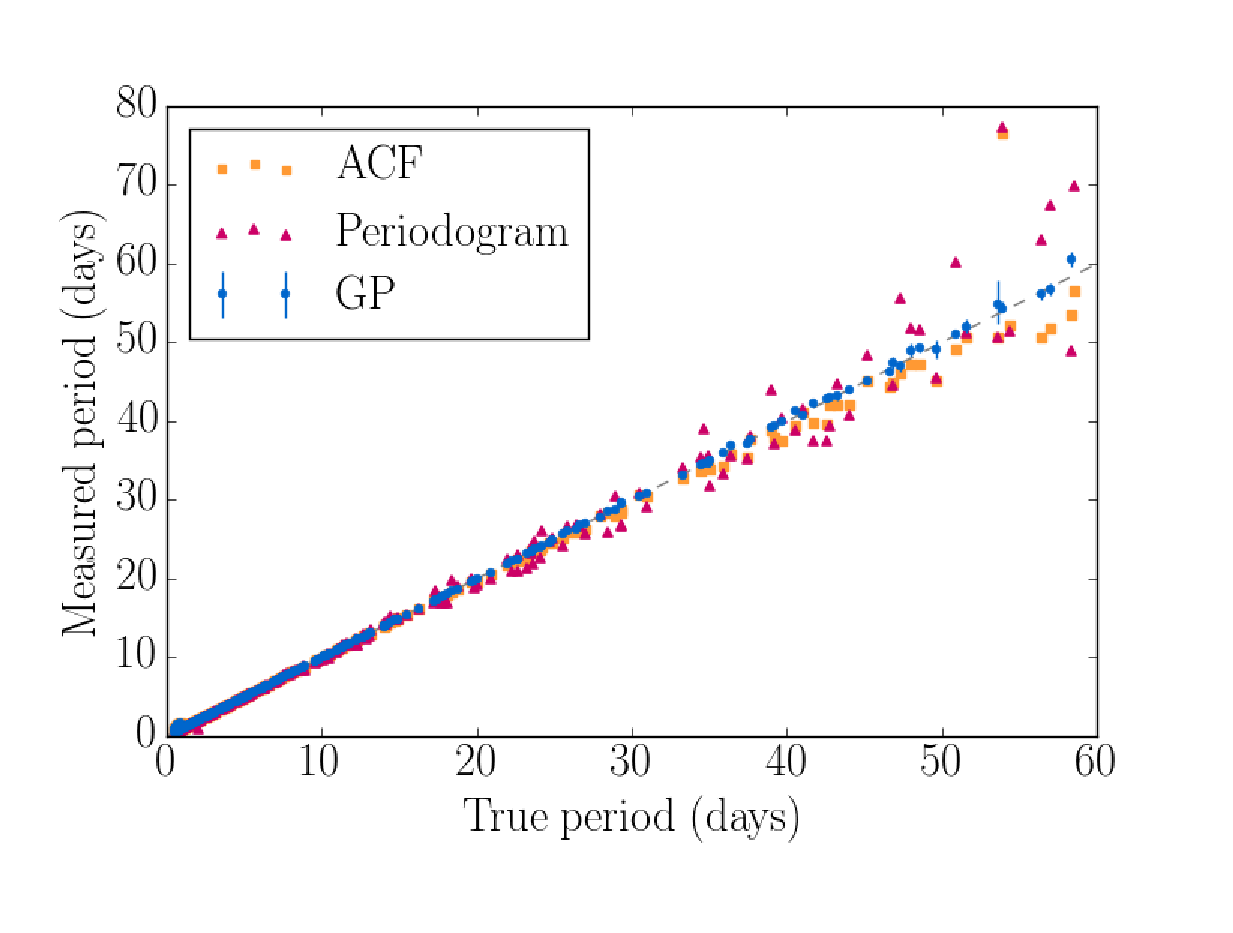
\includegraphics[width=3in,trim={0 1.2cm 0 1.2cm},clip]{compare2.eps}
% \vspace*{-1.0 cm}
 \caption{Measured vs true rotation periods for 300 simulations of light curves
	 from spotted, rotating stars.
	 Three different methods were tested: the ACF method, a Lomb-Scargle
	 periodogram (sine-fitting) method and our new GP method.
	 The GP method measures the most precise and accurate rotation periods
	 and is expected to perform even better on real data.}
   \label{fig1}
\end{center}
\end{figure}

% \begin{thebibliography}

% \bibitem[Mcquillan {\it et al.} (2014)]{amy}
% McQuillan, A., Mazeh, T. \& Aigrain, S., ApJ, 211, 24

% \bibitem[Foreman-Mackey {\it et al.} (2013)]{emcee}
% Foreman-Mackey, D., Hogg, D.~W., Lang, D., Goodman, J., 2013, PASP, 125, 306

% \bibitem[Foreman-Mackey (2015)]{george}
% Foreman-Mackey, D.

% \end{thebibliography}

\end{document}
